\hypertarget{GUIAnalyzePointWindow_8cpp}{\section{/daten/\-Projekte/eclipse\-\_\-workspace/simpleanalyzer-\/gui/src/\-G\-U\-I/\-G\-U\-I\-Analyze\-Point\-Window.cpp-\/\-Dateireferenz}
\label{GUIAnalyzePointWindow_8cpp}\index{/daten/\-Projekte/eclipse\-\_\-workspace/simpleanalyzer-\/gui/src/\-G\-U\-I/\-G\-U\-I\-Analyze\-Point\-Window.\-cpp@{/daten/\-Projekte/eclipse\-\_\-workspace/simpleanalyzer-\/gui/src/\-G\-U\-I/\-G\-U\-I\-Analyze\-Point\-Window.\-cpp}}
}
{\ttfamily \#include \char`\"{}G\-U\-I\-Analyze\-Point\-Window.\-h\char`\"{}}\\*
{\ttfamily \#include $<$iostream$>$}\\*
{\ttfamily \#include $<$sstream$>$}\\*
{\ttfamily \#include \char`\"{}constants.\-h\char`\"{}}\\*
{\ttfamily \#include \char`\"{}../processing/\-Analyzer.\-h\char`\"{}}\\*
{\ttfamily \#include \char`\"{}../\-Simple\-Analyzer\-App.\-h\char`\"{}}\\*
Include-\/\-Abhängigkeitsdiagramm für G\-U\-I\-Analyze\-Point\-Window.\-cpp\-:
\nopagebreak
\begin{figure}[H]
\begin{center}
\leavevmode
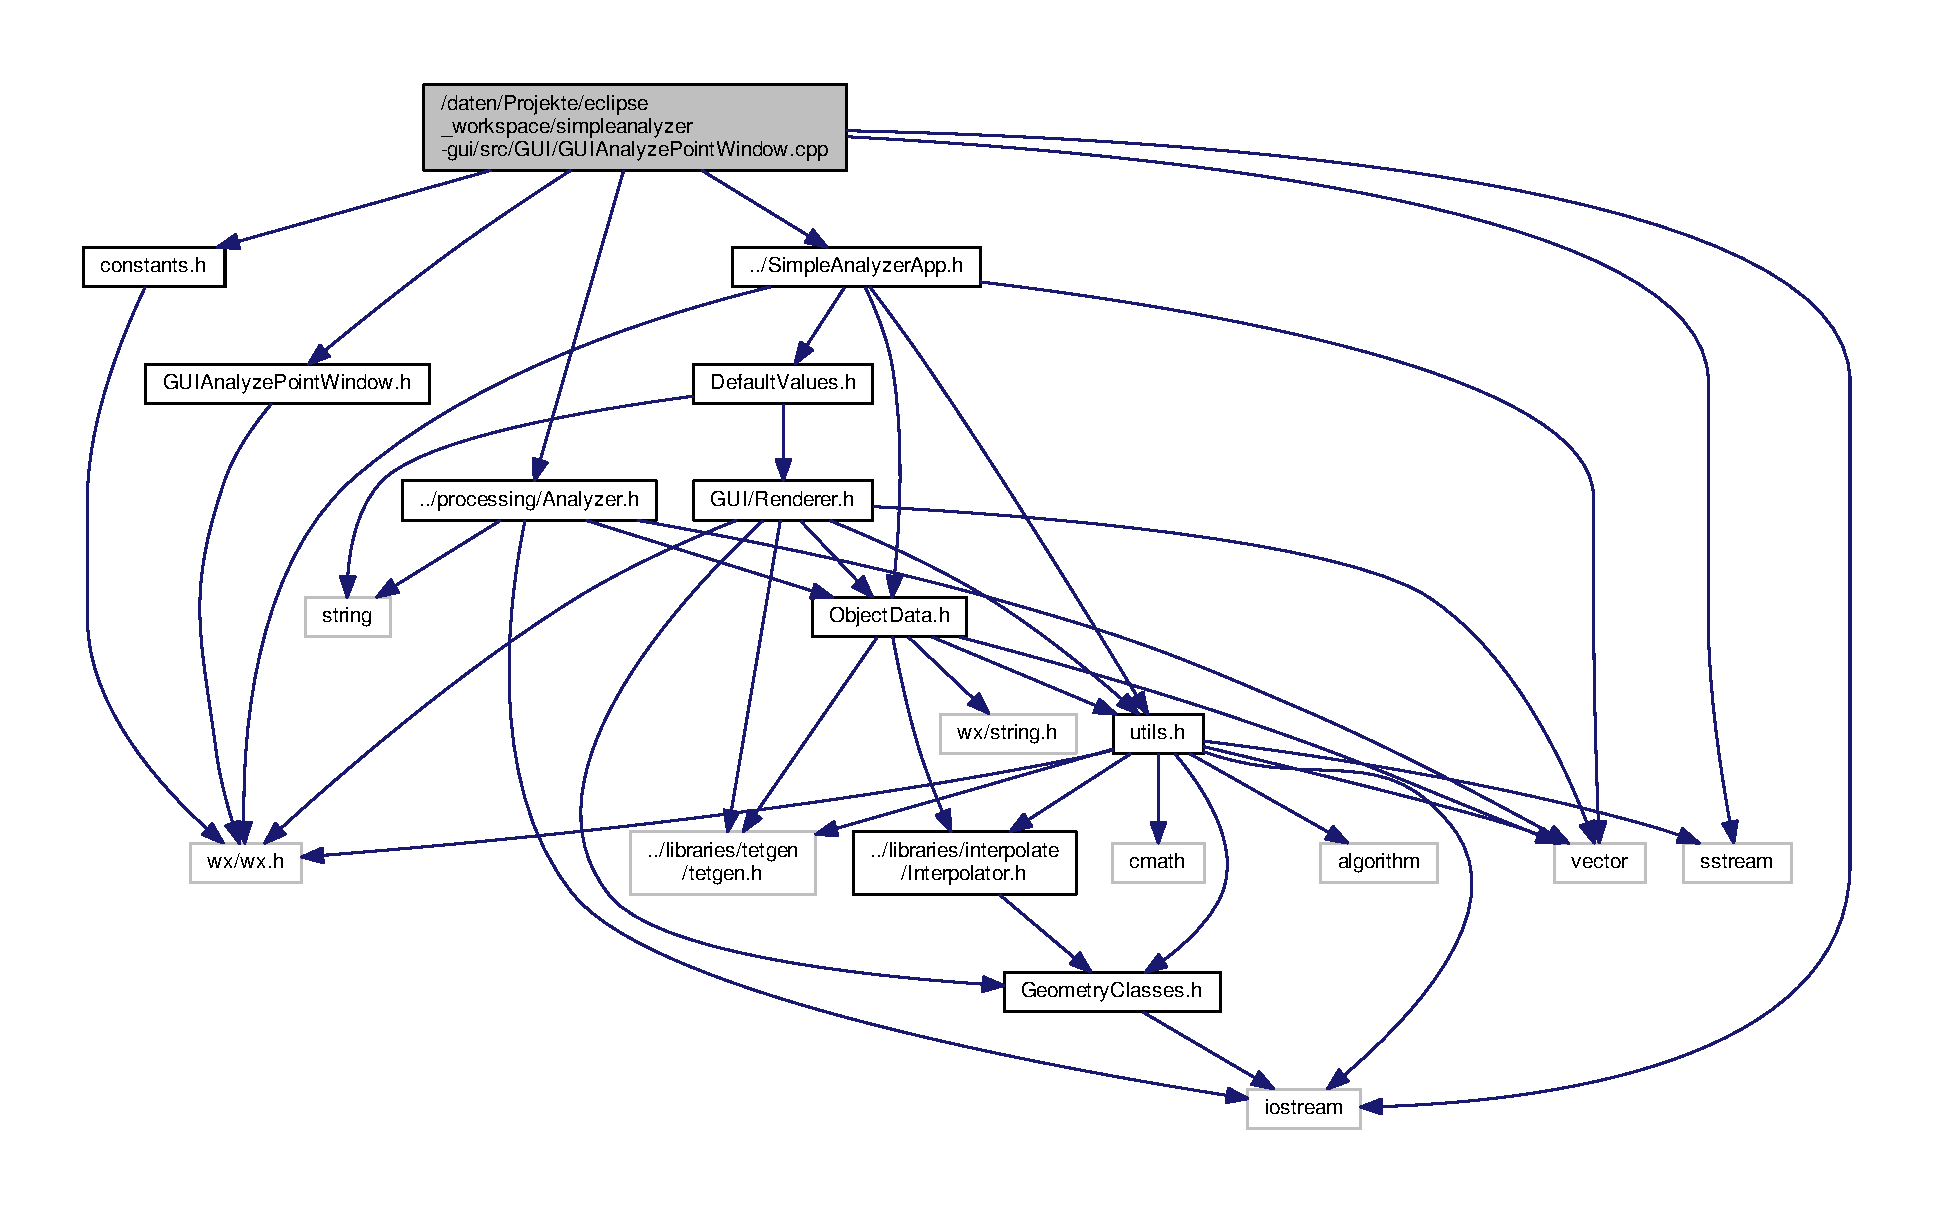
\includegraphics[width=350pt]{GUIAnalyzePointWindow_8cpp__incl}
\end{center}
\end{figure}
